%!TEX root = da-screen.tex

\section{Introduction}

As a running example in this chapter, we will use the following task: find a $3$-colouring of a directed cycle in the model of unique identifiers.

In a \emph{directed cycle}, we assume that we are given a graph $G = (V,E)$ that is an orientation of a cycle graph. In particular, we assume that each node $v \in V$ has
\[
    \outdegree_G(v) = \indegree_G(v) = 1,
\]
that is, there is precisely one incoming edge and one outgoing edge. Without loss of generality, we will assume that the incoming edge is connected to port number 1 and the outgoing edge is connected to port number 2 in each node \mydash if this was not the case, each node could renumber its ports locally. See Figure~\ref{fig:directed-cycle} for an illustration.

\begin{figure}
    \centering
    \includegraphics[page=\PDirectedCycle]{figs.pdf}
    \caption{A directed cycle with unique identifiers.}\label{fig:directed-cycle}
\end{figure}

Clearly, directed cycles are a special case of directed pseudoforests, and we already know how to find a $3$-colouring of a directed pseudoforest in the model of unique identifiers. Indeed, there are several possible strategies.
\begin{itemize}
    \item The greedy algorithm is simple but slow; in the case of directed cycles, it requires $\Omega(n)$ rounds in the worst case.
    \item Algorithm $\algo{DPBit}$ is much faster\mydash as we saw in Exercise~\ref{ex:logstar}, algorithm $\algo{DPBit}$ finds a $6$-colouring in $O(\log^* n)$ rounds, and we can then use the greedy algorithm to reduce the number of colours from $6$ to $3$ in constant time.
    \item Algorithm $\algo{DPBit}$ is in no way unique, and there are many alternative strategies that we can use to $3$-colour a directed pseudoforest. Exercises \ref{ex:dpbit-base} and \ref{ex:dpset} explore some possible ideas.
\end{itemize}
Moreover, directed cycles are a simple special case of directed pseudoforests, and whenever we have an algorithm that finds a $3$-colouring in any directed pseudoforest, we can construct a slightly faster algorithm that finds a $3$-colouring in directed cycles\mydash for example, we can easily speed up algorithm $\algo{DPGreedy}$ by a factor of two in directed cycles, as the construction of intermediate colouring $s$ becomes unnecessary.

However, no matter what combination of algorithm ideas we use, it appears that the worst-case running time of the algorithm is always $\Omega(\log^* n)$. That is, the running time \emph{slightly} increases as the number of nodes $n$ increases.

In this chapter we will prove that this is indeed necessary. We show that there is no $O(1)$-time algorithm that $3$-colours any directed cycle in the model of unique identifiers.


\section{Speed Limits}\label{sec:speed-limits}

We will now use Ramsey's theorem to prove that directed cycles cannot be $3$-coloured in constant time.

\begin{theorem}\label{thm:colour-lb}
    Assume that $A$ is a distributed algorithm for the model of unique identifiers. Assume that there is a constant $T \in \NN$ such that $A$ stops in time $T$ in any directed cycle $G = (V,E)$, and outputs a labelling $g\colon V \to \{1,2,3\}$. Then there exists a directed cycle $G$ such that if we execute $A$ on $G$, the output of $A$ is not a proper vertex colouring of~$G$.
\end{theorem}

To prove Theorem~\ref{thm:colour-lb}, let $n = 2T+2$, $k = 2T+1$, and $c = 3$. By Ramsey's theorem, $R_c(n;k)$ is finite. Choose any $N \ge R_c(n;k)$.

We will construct a directed cycle $G = (V,E)$ with $N$ nodes. In our construction, the set of nodes is $V = \{1,2,\dotsc,N\}$. This is also the set of unique identifiers in our cycle; recall that we follow the convention that the unique identifier of a node $v \in V$ is $v$.

With the set of nodes fixed, we proceed to define the set of edges. In essence, we only need to specify in which order the nodes are placed along the cycle.

\subsection{Subsets and Cycles}

For each subset $X \subseteq V$, we define a directed cycle $G_X = (V,E_X)$ as follows; see Figure~\ref{fig:subset-cycle}. Let $\ell = |X|$. Label the nodes by $x_1, x_2, \dotsc, x_N$ such that
\begin{align*}
    X &= \Set{ x_1, x_2, \dotsc, x_{\ell} }, \\
    V \setminus X &= \Set{ x_{\ell+1}, x_{\ell+1}, \dotsc, x_N }, \\
    x_1 &< x_2 < \dotsb < x_{\ell}, \\
    x_{\ell+1} &< x_{\ell+1} < \dotsb < x_N.
\end{align*}
Then choose the edges
\[
    E_X = \Set{ (x_i, x_{i+1}) : 1 \le i < N } \, \cup \, \Set{ (x_N,x_1) }.
\]

\begin{figure}
    \centering
    \includegraphics[page=\PSubsetCycle]{figs.pdf}
    \caption{Construction of $G_X$. Here $N = 6$ and $X = \{2,4\}$.}\label{fig:subset-cycle}
\end{figure}

Informally, $G_X$ is constructed as follows: first take all nodes of $X$, in the order of increasing identifiers, and then take all other nodes, again in the order of increasing identifiers.


\subsection{Labelling}

If $B \subseteq V$ is a $k$-subset, then we define that the \emph{internal node} $i(B)$ is the median of the set $B$. Put otherwise, $i(B)$ is the unique node in $B$ that is not among the $T$ smallest nodes of $B$, nor among the $T$ largest nodes of $B$.

We will use algorithm $A$ to construct a $c$-labelling $f$ of $V^{(k)}$ as follows. For each $k$-subsets $B \subseteq V$, we construct the cycle $G_B$, execute $A$ on $G_B$, and define that $f(B)$ is the output of node $i(B)$ in $G_B$. See Figure~\ref{fig:colour-lb} for an illustration.

\begin{figure}
    \centering
    \includegraphics[page=\PColourLB]{figs.pdf}
    \caption{In this example, $N = 10$ and $T = 2$. Let $B = \Set{1,2,4,5,7}$, $C = \Set{2,4,5,7,9}$, and $X = \Set{1,2,4,5,7,9}$. The label $f(B)$ is defined as follows: we construct $G_B$, execute algorithm $A$, and take the output of the internal node $i(B) = 4$. Similarly, the label $f(C)$ is the output of node $i(C) = 5$ in $G_C$. As the local neighbourhoods are identical, the output of node $4$ in $G_X$ is also $f(B)$, and the output of node $5$ in $G_X$ is also $f(C)$. If $X$ is monochromatic in $f$, we have $f(B) = f(C)$.}\label{fig:colour-lb}
\end{figure}


\subsection{Monochromatic Subsets}

We have constructed a certain $c$-labelling $f$. As $N$ is sufficiently large, there exists an $n$-subset $X \subseteq V$ that is monochromatic in~$f$. Let us label the nodes of $X$ by
\[
    X = \{ x_0, x_1, \dotsc, x_k \},
\]
where $x_0 < x_1 < \dotsb < x_k$. Let
\begin{align*}
    B &= \{ x_0,x_1,\dotsc,x_{k-1} \}, \\
    C &= \{ x_1,x_2,\dotsc,x_k \}.
\end{align*}
See Figure~\ref{fig:colour-lb} for an illustration.

Sets $B$ and $C$ are $k$-subsets of $X$, and their internal nodes are $i(B) = x_{T}$ and $i(C) = x_{T+1}$. As $X$ is monochromatic, we have $f(B) = f(C)$. Therefore we know that the output of $x_{T}$ in $G_B$ equals the output of $x_{T+1}$ in $G_C$.

Moreover, node $x_{T}$ has isomorphic radius-$T$ neighbourhoods in $G_B$ and $G_X$; in both graphs, the radius-$T$ neighbourhood of node $x_{T}$ is a directed path, along which we have the nodes $x_0,x_1,\dotsc,\allowbreak x_{k-1}$ in this order. Hence by Theorem~\ref{thm:local-neighbourhood}, the output of $x_{T}$ in $G_B$ equals the output of $x_{T}$ in $G_X$.

A similar argument shows that the output of $x_{T+1}$ in $G_C$ equals the output of $x_{T+1}$ in $G_X$. In summary, the output of $x_{T}$ in $G_X$ equals $f(B)$, which equals $f(C)$, which equals the output of $x_{T+1}$ in $G_X$.

We have shown that in the directed cycle $G_X$, there are two adjacent nodes, $x_T$ and $x_{T+1}$, that produce the same output. Hence $A$ does not output a proper vertex colouring in $G_X$.


\section{Exercises}

\begin{ex}
    Prove that it is not possible to find a proper vertex colouring with at most $100$ colours in any directed cycle in constant time.

    \hint{You can modify the proof of Theorem~\ref{thm:colour-lb}. Alternatively, you can show that if you could find a $100$-colouring in constant time, you could also find a $3$-colouring in constant time.}
\end{ex}

\begin{ex}
    Prove that it is not possible to find a maximal independent set in any directed cycle in constant time.

    \hint{Assume that algorithm $A$ finds an independent set in time $T$ in any directed cycle. Follow the basic idea of the proof of Theorem~\ref{thm:colour-lb}. Choose $n = 2T+3$, $k = 2T+1$, and $c = 2$. Show that you can construct a cycle in which a node and \emph{both} of its neighbours produce the same output. Argue that if the output is a valid independent set, it cannot be a maximal independent set.}
\end{ex}

\begin{ex}
    Prove that it is not possible to find a maximal matching in any directed cycle in constant time.
\end{ex}

\begin{ex}\label{ex:is-apx-lb}
    Prove that it is not possible to find a \Apx{100} of a maximum independent set in any directed cycle in constant time.
    
    \hint{You will need several applications of Ramsey's theorem. First, choose a (very large) space of unique identifiers. Then apply Ramsey's theorem to find a large monochromatic subset, remove the set, and repeat. This way you have partitioned \emph{almost} all identifiers into monochromatic subsets. Each monochromatic subset is used to construct a fragment of the cycle.}
\end{ex}


\section{Bibliographic Notes}

Ramsey's theorem has been used to prove lower bounds on distributed algorithms by, e.g., Naor and Stockmeyer~\cite{naor95what} and Czygrinow et al.~\cite{czygrinow08fast}. In particular, the idea of Exercise~\ref{ex:is-apx-lb} is from Czygrinow et al.~\cite{czygrinow08fast}.
